\section{问题二的模型建立与求解}
\subsection{变物性热湿耦合模型}
沿用第一问的固定圆柱径向结构、初值和有效交换边界，将全时段物性统一替换为附录3。
本问从 $T(r,0)=28$、$C(r,0)=2.55$ 重新积分，不以第一问的1800 s末态为初值，因而两问结果不能直接拼接为同一条时间轨迹。
令 $B(C)=\rho(C)c_p(C)$，方程为
\begin{align}
B(C)T_t&=\frac1r\partial_r[rk(C)T_r],\label{eq:q2_heat}\\
C_t&=\frac1r\partial_r[rD(C,T)C_r],\label{eq:q2_moisture}\\
\rho(C)&=650+128C,\qquad c_p(C)=1450+2736\frac{C}{1+C},\\
k(C)&=0.21+0.38\frac{C}{1+C},\\
D(C,T)&=2.4\times10^{-3}\exp\left(-\frac{0.45}{C}\right)
\exp\left(-\frac{3850}{T+273.15}\right).
\end{align}
温度状态量以摄氏度存储，经验扩散系数中的温度换算为开尔文；其余物性单位与第一问相同。
中心仍采用零梯度条件，表面为
\begin{equation}
-k(C_s)T_r(R,t)=h(T_s-T_a),\qquad
-D(C_s,T_s)C_r(R,t)=h_m(C_s-C_a).
\end{equation}
由于局部温度影响 $D$，含水率又影响 $B$ 与 $k$，两场必须联合推进。
变系数保留在散度算子内，不将水分方程简化为 $D(C,T)(C_{rr}+C_r/r)$，以免遗漏系数空间变化的影响。
附录中的密度用于有效热容量，不另以 $\rho/(1+C)$ 构造可变干物质密度。
本问继续采用无显式潜热和忽略端面的等效模型。

\subsection{联合求解与验证}
对附件1中前3小时的181个环境节点采用PCHIP插值，节点全部保留，计算时段内无需外推。
径向控制体与第一问一致，$k$、$D$ 的面系数按局部状态更新，储热项采用 $B(C_i)W_i\dot T_i$。
温度和含水率组成联合状态向量，采用隐式BDF积分。
比较529与1057个节点后选用1057节点；独立审核进一步以2113节点检查完整3小时结果。
生产相对容差为 $10^{-9}$，温度和含水率绝对容差为 $10^{-8}$、$10^{-10}$，最大时间步长为1 s；另进行容差缩小5倍和最大步长0.5 s的复算。

独立加密检查中，1057与2113节点的全部规定输出点温度、含水率最大差分别为
$6.24\times10^{-7}\,^\circ\mathrm C$、$3.73\times10^{-6}\,\mathrm{kg/kg}$。
论文两表共60个四位小数在时间与空间加密后均不变。
另以预先给定的光滑温湿场反推源项，进行变系数制造解检验，温度、含水率最大误差分别为 $6.09\times10^{-8}$、$8.98\times10^{-9}$。
冻结 $D$ 的辅助水分问题采用Bessel参考，级数加倍后再比较，避免早期级数截断不足影响判断。

水分收支以径向权重加权存量与表面通量积分核对。
对热方程，定义有效储热量
\begin{equation}
E(t)=2\pi L\int_0^R B(C)(T-28)r\,\mathrm dr.
\end{equation}
由乘积求导可得
\begin{equation}
E(t)-E(0)-2\pi L\int_0^t\!\int_0^R
B'(C)(T-28)C_t r\,\mathrm dr\,\mathrm d\tau
=2\pi RL\int_0^t h(T_a-T_s)\,\mathrm d\tau.
\end{equation}
该组成修正项来自乘积求导，不能省略。
热、湿相对收支残差分别为 $3.57\times10^{-8}$、$4.31\times10^{-7}$；全部内部节点满足所设温湿界限。
这一有效热收支不是包含潜热和组分焓输运的完整物理能量守恒。

\subsection{前三小时的干燥规律}

\begin{table}[H]
\centering
\caption{3小时内药材温度（$^\circ\mathrm C$）}\label{tab:q2_T}
\small
\begin{tabular}{rrrrrr}
\toprule
时间/h & \multicolumn{5}{c}{到中心的距离/cm}\\
\cmidrule(lr){2-6}
 & 0 & 0.5 & 1.0 & 1.5 & 2.0\\
\midrule
0.5 & 32.1896 & 32.3824 & 32.9660 & 33.9608 & 35.4132 \\
1.0 & 40.3822 & 40.5542 & 41.0609 & 41.8783 & 43.0000 \\
1.5 & 45.8471 & 45.9351 & 46.1932 & 46.6055 & 47.1397 \\
2.0 & 48.4503 & 48.4881 & 48.5985 & 48.7736 & 49.0033 \\
2.5 & 49.4670 & 49.4793 & 49.5136 & 49.5645 & 49.6617 \\
3.0 & 49.8494 & 49.8553 & 49.8746 & 49.9096 & 49.9645 \\
\bottomrule
\end{tabular}
\end{table}

\begin{table}[H]
\centering
\caption{3小时内药材干基含水率（kg/kg）}\label{tab:q2_C}
\small
\begin{tabular}{rrrrrr}
\toprule
时间/h & \multicolumn{5}{c}{到中心的距离/cm}\\
\cmidrule(lr){2-6}
 & 0 & 0.5 & 1.0 & 1.5 & 2.0\\
\midrule
0.5 & 2.5499 & 2.5489 & 2.5256 & 2.3257 & 1.6486 \\
1.0 & 2.5257 & 2.4948 & 2.3578 & 2.0230 & 1.4711 \\
1.5 & 2.3861 & 2.3256 & 2.1344 & 1.8020 & 1.3476 \\
2.0 & 2.1708 & 2.1084 & 1.9236 & 1.6259 & 1.2311 \\
2.5 & 1.9566 & 1.9006 & 1.7360 & 1.4720 & 1.1166 \\
3.0 & 1.7662 & 1.7165 & 1.5702 & 1.3333 & 1.0081 \\
\bottomrule
\end{tabular}
\end{table}
3 h时，中心与表面温度分别为 $49.8494\,^\circ\mathrm C$、$49.9645\,^\circ\mathrm C$，
温差约 $0.1151\,^\circ\mathrm C$，而两处干基含水率仍分别为 $1.7662$ 和 $1.0081$。
温度已接近烘房恒温水平，水分仍存在显著径向差异，说明热平衡与干燥完成不是同一条件。
该时刻尚未满足各处含水率低于 $0.15\,\mathrm{kg/kg}$ 的要求。

\begin{figure}[H]
\centering
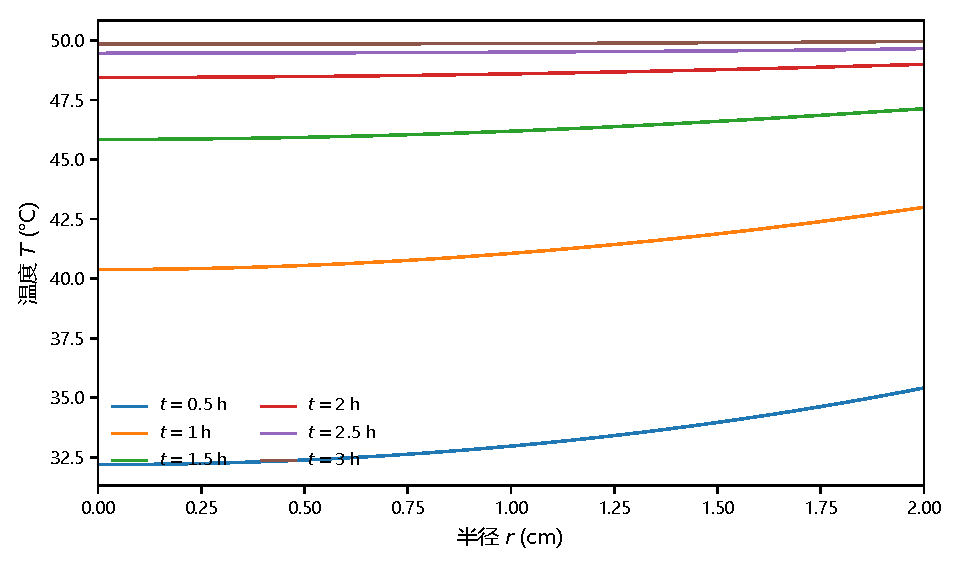
\includegraphics[width=.70\textwidth]{../figures/q2_T_profiles.pdf}
\caption{前三小时不同时间的径向温度分布}\label{fig:q2_T}
\end{figure}

\begin{figure}[H]
\centering
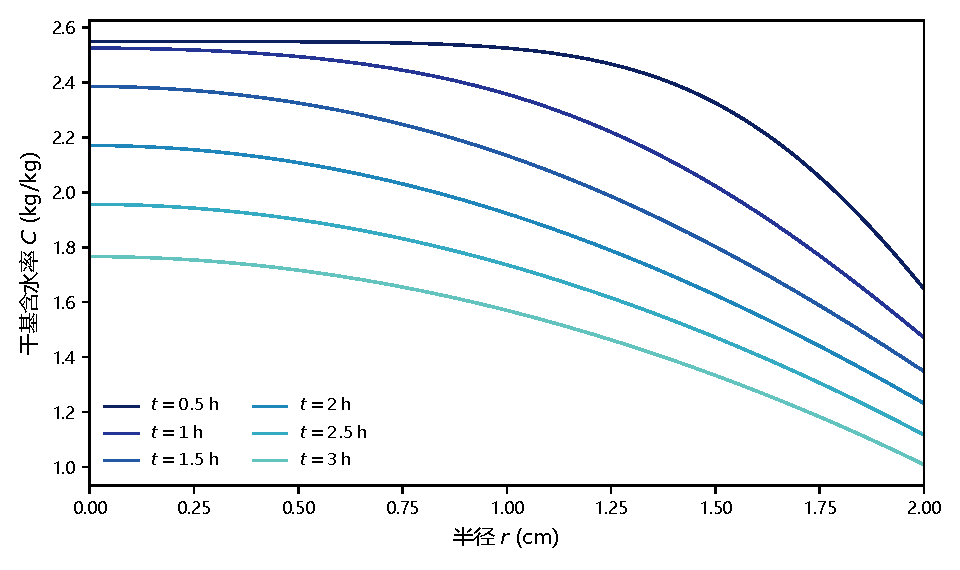
\includegraphics[width=.70\textwidth]{../figures/q2_C_profiles.pdf}
\caption{前三小时不同时间的径向干基含水率分布}\label{fig:q2_C}
\end{figure}
经验式中，升温使扩散系数增大，含水率下降则使扩散系数减小。
这两种作用随时间与位置共同变化，因此不能用固定扩散系数或前三小时的失水斜率直接外推最终干燥时长。
本问将前3小时每隔1 s、径向每隔 $0.1\,\mathrm{cm}$ 的温度和含水率写入 \texttt{result2.xlsx}。
内部计算网格比输出网格更细，保存初值、论文表时刻和末态检查点以便复核。
后续长时预测仍需单独明确环境延续，并检验长期一维近似与达标时刻的数值稳定性。
